%%%%%%%%%%%%%%%%%%%%%%%%%
% Dokumentinformationen %
%%%%%%%%%%%%%%%%%%%%%%%%%
\title{JavaC - CheatSheet}
\author{\href{mailto:jan.brupbacher@hsr.ch}{J. Brupbacher}}
\newcommand{\authoremail}{\href{mailto:jan.brupbacher@hsr.ch}{jan.brupbacher@hsr.ch} }
\newcommand{\versioninfo}{$ V1.1 $}

\documentclass[10pt,twoside,a4paper,fleqn]{scrartcl}
%%%%%%%%%%%%%%%%%%%%%%%%%%%%%%%%%%%%%%%%%%%%%
% Standard Header für 
% - Makros 
% - Farben
% - Mathematische Operatoren
%%%%%%%%%%%%%%%%%%%%%%%%%%%%%%%%%%%%%%%
%% Makros & anderer Low-Level bastel %%
%%%%%%%%%%%%%%%%%%%%%%%%%%%%%%%%%%%%%%%
\makeatletter
%% Makros für Titel, Autor und Datum 
%% Dank diesem Makro stehen Titel, Autor und Datum überall im Dokument zur verfügung
%% Date hat zudem den Default-Wert \today
\def\@Title{}
\def\@Author{}
\def\@Date{\today}
\newcommand{\Title}{\@Title}
\newcommand{\Author}{\@Author}
\newcommand{\Date}{\@Date}
\AtBeginDocument{%
  \let\@Title\@title
  \let\@Author\@author
  \let\@Date\@date
}

%% Makros für den Arraystretch (bei uns meist in Tabellen genutzt, welche Formeln enthalten)
% Default Value
\def\@ArrayStretchDefault{1} % Entspricht der Voreinstellung von Latex

% Setzt einen neuen Wert für den arraystretch
\newcommand{\setArrayStretch}[1]{\renewcommand{\arraystretch}{#1}}

% Setzt den arraystretch zurück auf den default wert
\newcommand{\resetArrayStretch}{\renewcommand{\arraystretch}{\@ArrayStretchDefault}}

% Makro zum setzten des Default arraystretch. Kann nur in der Präambel verwendet werden.
\newcommand{\setDefaultArrayStretch}[1]{%
	\AtBeginDocument{%
		\def\@ArrayStretchDefault{#1}
		\renewcommand{\arraystretch}{#1}
	}
}
\makeatother


%%%%%%%%%%%%%%%%%%%%%%%
%% Wichtige Packages %%
%%%%%%%%%%%%%%%%%%%%%%%
\usepackage[utf8]{inputenc} % UTF-8 unterstützung
\usepackage[english, ngerman]{babel} % Silbentrennung
\usepackage[automark]{scrpage2} % Header und Footer
\usepackage{tabularx}

% Für Abbildungen mit mehreren kleinen Bilder
% Doku: http://www.ctan.org/tex-archive/macros/latex/contrib/caption/
\usepackage[justification=centering]{caption}
\usepackage{subcaption}

\ifx\GUARDlistings\undefined
\def\GUARDlistings{}

\usepackage{color}

\definecolor{mygreen}{rgb}{0,0.6,0}
\definecolor{mygray}{rgb}{0.5,0.5,0.5}
\definecolor{mymauve}{rgb}{0.58,0,0.82}
\definecolor{bgGray}{rgb}{0.9,0.9,0.9}
\definecolor{myorange}{rgb}{1, 0.3, 0}
\definecolor{numberBlue}{rgb}{0.4, 0.7, 1}

\usepackage{listings}
\lstset{ %
    firstnumber=1,
    backgroundcolor=\color{gray!15},   % choose the background color; you must add        \usepackage{color} or \usepackage{xcolor}
    basicstyle=\normalsize\ttfamily, % the size of the fonts that are used for the code
    breakatwhitespace=false,         % sets if automatic breaks should only happen at whitespace
    breaklines=true,                 % sets automatic line breaking
    captionpos=b,                    % sets the caption-position to bottom
    commentstyle=\color{mygreen},    % comment style
    deletekeywords={...},            % if you want to delete keywords from the given language
    otherkeywords={},             % if you want to add more keywords to the set
    escapeinside={\%*}{*\%},          % if you want to add LaTeX within your code
    extendedchars=true,              % lets you use non-ASCII characters; for 8-bits encodings only, does not work with UTF-8
    frame=tb,	                 % adds a frame around the code
    keepspaces=true,                 % keeps spaces in text, useful for keeping indentation of code (possibly needs columns=flexible)
    keywordstyle=\color{blue},       % keyword style
    language=C++,                    % the language of the code   
    numbers=none,                    % where to put the line-numbers; possible values are (none, left, right)
    numbersep=5pt,                   % how far the line-numbers are from the code
    numberstyle=\tiny\color{mygray}, % the style that is used for the line-numbers
    rulecolor=\color{black},         % if not set, the frame-color may be changed on line-breaks within not-black text (e.g. comments (green here))
    showspaces=false,                % show spaces everywhere adding particular underscores; it overrides 'showstringspaces'
    showstringspaces=false,          % underline spaces within strings only
    showtabs=false,                  % show tabs within strings adding particular underscores
    stepnumber=2,                    % the step between two line-numbers. If it's 1, each line will be numbered
    stringstyle=\color{mymauve},     % string literal style
    tabsize=4,	                     % sets default tabsize to 2 spaces
    %title=\lstname                   % show the filename of files included with         \lstinputlisting; also try caption instead of title
}

\lstdefinestyle{Java}{
	belowcaptionskip=1\baselineskip,
	breaklines=true,
	language=Java,
	showstringspaces=false,
	otherkeywords={@Override, var},
	keywordstyle=\color{myorange},
	commentstyle=\color{mymauve},
	identifierstyle=\color{black},
	stringstyle=\color{mygreen},
	numberstyle=\color{numberBlue},
	tabsize=4
}

\lstdefinestyle{C}{
  numbers=left,
  belowcaptionskip=1\baselineskip,
  breaklines=true,
  frame=L,
  xleftmargin=10pt,
  language=C,
  showstringspaces=false,
  basicstyle=\footnotesize\ttfamily,
  keywordstyle=\bfseries\color{green!40!black},
  commentstyle=\itshape\color{purple!40!black},
  identifierstyle=\color{blue},
  stringstyle=\color{orange},
  numberstyle=\ttfamily\tiny,
  tabsize=2
}

\lstdefinestyle{Cpp}{
  numbers=left,
  belowcaptionskip=1\baselineskip,
  breaklines=true,
  frame=L,
  xleftmargin=10pt,
  language=C++,
  showstringspaces=false,
  basicstyle=\footnotesize\ttfamily,
  keywordstyle=\bfseries\color{green!40!black},
  commentstyle=\itshape\color{purple!40!black},
  identifierstyle=\color{blue},
  stringstyle=\color{orange},
  numberstyle=\ttfamily\tiny,
  tabsize=2
}

% Seitenränder
\usepackage[left=1cm,right=1cm,top=0.5cm,bottom=0.5cm,includeheadfoot]{geometry}

\usepackage{hyperref}
\usepackage{longtable}
\usepackage{multirow} % Create tabular cells spanning multiple rows
\usepackage{multicol} % In­ter­mix sin­gle and mul­ti­ple columns
\usepackage{rotating} % Rotation tools, including rotated fullpage floats
\usepackage{enumitem}
\usepackage{graphicx}
\usepackage{graphbox} % Align Images
\usepackage{bold-extra} % for usage of both \textbf and \texttt on one word
\usepackage[export]{adjustbox}	% Align Images 

%%%%%%%%%%%%%%%%%%%%%%%%%%%%%%%%%%%
%% Layout der Kopf und Fusszeile %%
%%%%%%%%%%%%%%%%%%%%%%%%%%%%%%%%%%%
\deftripstyle{zusammenfassung}[0pt][0.5pt]
	{\Title}	% Kopfzeile innen
	{HS19}	% Kopfzeile mitte
	{\pagemark}	% Kopfzeile aussen
	{\Author}	% Fusszeile innen
	{
\includegraphics[width=1.6cm]{./header/lizenzen/cc-by-nc-sa/small.png}}			% Fusszeile mitte
	{\Date}	% Fusszeile aussen
\pagestyle{zusammenfassung}

% Nummerierte und unnummerierte paragraph headings
\setcounter{secnumdepth}{5}

\RedeclareSectionCommands[
  afterskip=1em
]{paragraph,subparagraph}

\renewcommand*{\paragraphformat}{\theparagraph\autodot\enskip}
\renewcommand*{\subparagraphformat}{\thesubparagraph\autodot\enskip}


%%Makros%%%%%%%%%%%%%%%%%%%%%%%%%%%%%%%%%%%%%%%%%%%  
% Command for images in table
\newcommand\tabImg[2][]{%
    \raisebox{0pt}[\dimexpr\totalheight+\dp\strutbox\relax][\dp\strutbox]{%
        \includegraphics[#1]{#2}%
    }%
}

% Zeilenhöhe Tabellen:
\newcommand{\arraystretchOriginal}{1.5}
\renewcommand{\arraystretch}{\arraystretchOriginal}

\setlength{\parindent}{0pt}

% Todo command
\newcommand{\todo}[1]{\textbf{\color{red}{TO DO: #1}}}
%%%%%%%%%%%%%%%%%%%%%%%%%%%%%%%%%%%%%%%%%%%%%
%Ergänzungen für Package kommen hier hin:
%\usepackage{hyperref}

\usepackage[table]{xcolor}
\renewcommand{\familydefault}{\sfdefault}

%%%%%%%%%%%%%%%%%%%%%%%%%%%%%%%%%%%%%%%%%%%%%%%%%%%%%%%%%%%%%%%%%%%%%%%%%%%%%%%%%%%%%%%%%%%%
%%%%%%%%%%%%%%%%%%%%%%%%%%%%%%%%%%%%%%%%%%%%%%%%%%%%%%%%%%%%%%%%%%%%%%%%%%%%%%%%%%%%%%%%%%%%

\begin{document}
\lstset{style=Java} 
\textbf{\huge{JavaC - CheatSheet}}\\
\vspace{-0.5cm}
\section*{Allgemein}
	\begin{minipage}[t]{10cm}
		\subsection*{Primitive Datentypen}
			\rowcolors{1}{gray!15}{white}
			\begin{tabular}{|>{\bfseries}l l l|}
				\hline   boolean & Boolescher Wert & true, false
				\\\hline char & Textzeichen (UTF16) & 'a', 'B', '0', 'é' etc.
				\\\hline byte & Ganzzahl (8 Bit) & -128 bis 127
				\\\hline short & Ganzzahl (16 Bit) & -32'768 bis 32'767
				\\\hline int & Ganzzahl (32 Bit) & -2$^{31}$ bis 2$^{31}$-1
				\\\hline long & Ganzzahl (64 Bit) & -2$^{63}$ bis 2$^{63}$-1, 1L (L Suffix)
				\\\hline float & Gleitkommazahl(32 Bit) & 0.1f, 2e4f (2*10$^4$)
				\\\hline double & Gleitkommazahl(64 Bit) & 0.1, 2e4 
				\\\hline
			\end{tabular}
		\end{minipage}
		\hspace*{0.6cm}
		\begin{minipage}[t]{8.4cm}
			\vspace*{0.7cm}
			\textbf{Überlauf/Unterlauf} ist in Java definiert. Zählt einfach, je nach dem, unten oder oben weiter. Bei Gleitkommazahlen wird 2*1e308 zu POSITIVE\_INFINITY.
			\subsection*{Explizite Typkonversation}
			Nur C-Style Cast: (int)3.5; $\rightarrow$ 3
			\\\todo{evtl. noch Arrays und Mehrdimensionale Arrays}
		\end{minipage}
	
	\vspace{0.3cm}\todo{evtl. komplexe Datentypen}
	\vspace{0.3cm}
	\lstinputlisting{code/test.java}
\section*{Collections}
	Collection sind Datenstrukturen für Gruppen von Elementen und forderne einen Import aus dem Packet java.util
	\subsection*{List}
	\begin{minipage}[t]{11cm}
			Eine Liste ist eine Folge von Elementen und kann wie folgt definiert werden:
			\lstinputlisting{code/ArrayList_definition.java}
	\end{minipage}
	\hspace*{0.5cm}
	\begin{minipage}[t]{7.3cm}
		\vspace*{-0.18cm}
		\paragraph*{Iteration mit Enhanced for}
			Besucht jedes Element in einer Collection:
			\lstinputlisting{code/foreach_example.java}
	\end{minipage}
	Einige nützliche Operationen mit Listen:
	\lstinputlisting{code/ArrayList_example.java}
	\subsection*{Set}
		Ein Set ist eine Menge von Elementen, in welchem jedes Element genau einmal vorkommt und wird wie folgt verwendent:
		\lstinputlisting{code/Set_example.java}
		
\section*{Map}
		Abbildung Schlüssel $\rightarrow$ Werte
		\lstinputlisting{code/Map_example.java}
		
\section*{Wrapper-Klassen}
	Collections (bzw. alle Generics) nehmen nur Referenzen, welche primitive Datentypen nicht bringen. Um dennoch int's oder double's in Listen zu speichern, gibt es sogenannte Wrapper-Klassen.\\
	\begin{minipage}[t]{10cm}
		\lstinputlisting{code/Wrapper_AutoBoxing.java}
	\end{minipage}
	\hspace*{0.5cm}
	\begin{minipage}[b]{7.3cm}
		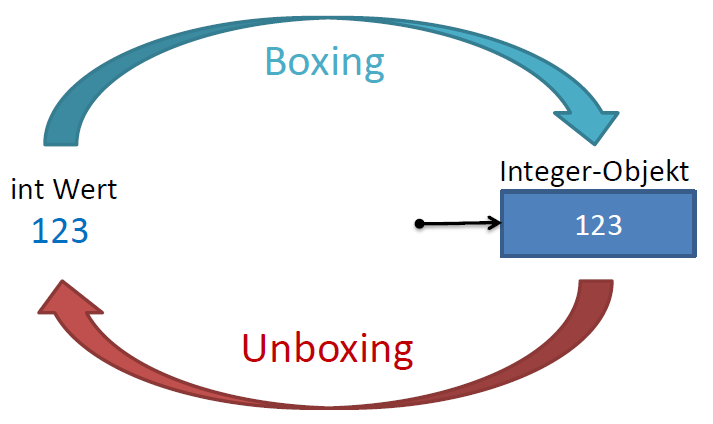
\includegraphics[height=2.5cm, align=t]{pics/boxing_unboxing.PNG}
	\end{minipage}
\section*{Vererbung}
	In Java gibt es nur Einfachvererbung, sprich jede Klasse hat maximal eine Basisklasse. Die Subklasse bietet alles was Superklasse bietet und eventuell mehr.\\
	\begin{minipage}[t]{8cm}
		\subsection*{Root Class Object}
		Jede Klasse erbt automatisch (direkt oder indirekt) von der obersten Basisklasse \texttt{Object}. Folgend einige der wichtigsten Methoden der Klasse \texttt{Object}:
		\lstinputlisting{code/Object_Member.java}
		\section*{Typ-Polymorphismus}
		Ein Objekt hat nicht nur den Typ seiner Klasse, sondern auch die Typen seiner Superklassen. Beispiel:
		\begin{minipage}[t]{5cm}
			\lstinputlisting{code/Typ_Polymorphismus.java}
			\todo{evtl. @override??}
		\end{minipage}
		\hspace*{0.5cm}
		\begin{minipage}[b]{2.3cm}
			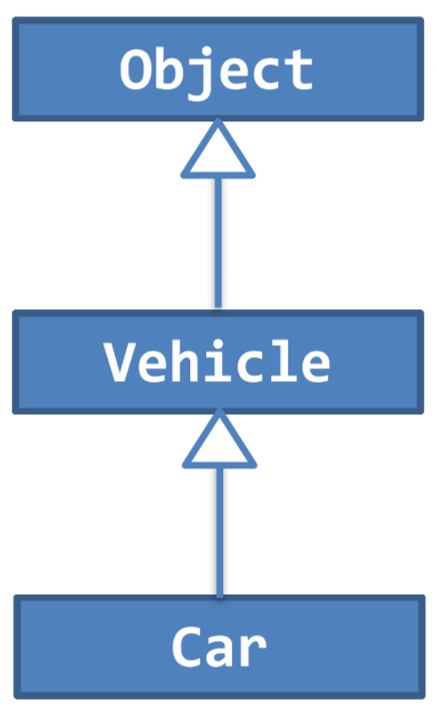
\includegraphics[height=3.8cm, align=t]{pics/Typ_Polymorphismus.PNG}
		\end{minipage}
	\end{minipage}
	\hspace*{0.5cm}
	\begin{minipage}[t]{10.3cm}
		\subsection*{Konstruktor bei Vererbung}
			Das erste Statement in jedem Konstruktor ist der Aufruf des Basis-Konstruktors mittels \texttt{super()}. Dieser wird implizit vom Compiler eingefügt, wenn ein Default-Konstruktor(ohne Parameter) existiert, ansonsten muss er an \textbf{erster} Stelle im Konstruktor explizit aufgerufen werden.
			\lstinputlisting{code/super_Explicit.java}
	\end{minipage}

	
	
\section*{Schnittstellen(Interfaces)}
	Ein Interface beschreibt die öffentlich nutzbare Funktionalität einer Klasse. Während aber Klassen instanziierbar sind, sind Interfaces lediglich als deklarierbare Typen verwendbar. \todo{evtl beispiel???}\\
	\begin{minipage}[t]{8.3cm}
		\subsection*{Spezifikation}
			\lstinputlisting{code/Interface_definition.java}
			Methoden einer Schnittstelle sind implizit \textbf{\texttt{public}} und \textbf{\texttt{abstract}}, sprich diese modifier können weggelassen werden. Andere Modifier sind ungültig.
		\subsection*{Kontstanten in Schnittstellen}
			\lstinputlisting{code/Interface_constant.java}
			Vermeintliche Variablen sind in Schnittstellen Konstanten, welche bei gutem Stil in Grossbuchstaben geschrieben werden. Diese sind implizit \textbf{\texttt{public}}, \textbf{\texttt{static}} und \textbf{\texttt{final}}.
		\todo{default Methoden!!!}
	\end{minipage}
	\hspace*{0.5cm}
	\begin{minipage}[t]{10cm}
		\subsection*{Implementation}
			\lstinputlisting{code/Interface_Implementation.java}
		\subsection*{Vererbungen und Mehrfachimplementation}
			\lstinputlisting{code/Interface_inheritance.java}
	\end{minipage}
	\subsection*{Kollisionen bei Mehrfach-Implementation}
	\textbf{gleiche Methode:} Methode wird nur einmal implementiert $\rightarrow$ kein Problem\\
	\textbf{gleichnamige Konstanten:} Muss explizit auf Konstante zugegriffen werden $\rightarrow$ \lstinline|Vehicle.HIGHWAY_MIN_SPEED|
	
\section*{Variadische Funktionen mit Varargs}
	\begin{minipage}[t]{7.3cm}
		\begin{itemize}[noitemsep]
			\item Erlaubt beliebige Anzahl Parameter
			\item Nur am Schluss der Parameterliste erlaubt
			\item Compiler generiert ein Array
	\end{itemize}
	\lstinputlisting{code/varargs_call.java}
	\end{minipage}
	\hspace*{0.5cm}
	\begin{minipage}[t]{11cm}
		\vspace*{-0.2cm}
		\lstinputlisting{code/varargs_definition.java}
	\end{minipage}
\newpage
\section*{Spezielle Grundfunktionen}
Grundfunktionen sind Funktionen, welche in jedem \texttt{Object()} vorhanden sind und nach bedarf überschrieben werden können.
	\subsection*{Gleichheit}
		\texttt{equals()} ist standardmässig nur \textbf{Referenzvergleich}. Für einen inhaltlichen Vergleich muss \texttt{equals()} überschrieben werden. \todo{sollte das immer der Fall sein?} Bei der \texttt{String} Klasse ist es bereits implementiert, bei Arrays aber nicht!
	\lstinputlisting{code/equals.java}
	\subsection*{Hash-Code}
		\begin{itemize}[noitemsep]
			\item Sobald \texttt{equals()} überschrieben wird, muss auch \texttt{hashCode()} überschrieben werden.
			\item \texttt{hash-Code()} berechnet aus Objektinhalt den Hash-Code.
			\item Hashcodes müssen immer gleich sein, wenn Objekte equals sind.
			\item Umkehrung muss nicht umbedingt gelten!
			\item Mittels \textbf{Hashing} kann ein Element effizient gefunden werden.\vspace*{-0.15cm}
			\begin{itemize}[noitemsep]
				\item \textbf{Streuspeicher}: Elemente werden auf ein Array(Hash-Tabelle) verstreut, mit 'Hash-Code' als jeweiliger Index.
			\end{itemize}
		\end{itemize}
		\begin{minipage}[t]{8cm}
			\textbf{Eigene Hashfunktion:}
			\lstinputlisting{code/hashCode.java}
			Die Erstellung von \texttt{hashCode()} und \texttt{equals()} wird üblicherweise der IDE überlassen.
		\end{minipage}
		\hspace*{0.5cm}
		\begin{minipage}[t]{9.3cm}
			\textbf{Beispiel:}\\
			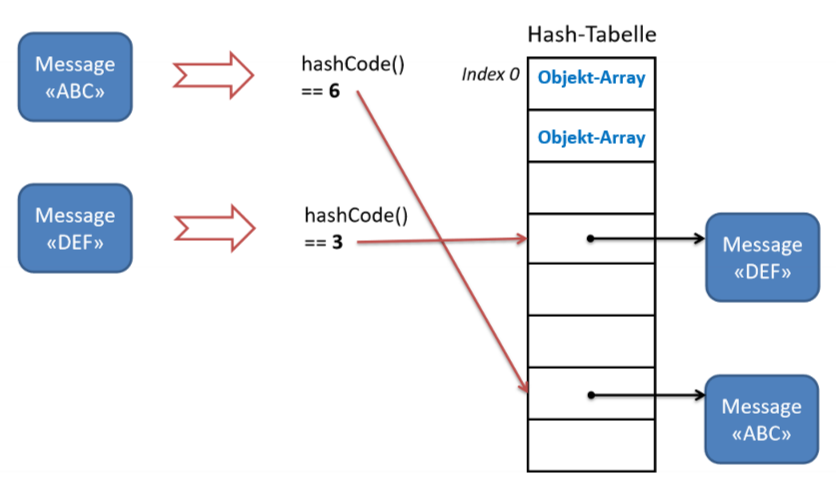
\includegraphics[height=6cm, align=t]{pics/hashing.PNG}
		\end{minipage}
		
\section*{Generics}
	Generics sind zu vergleichen mit Templates in \texttt{C++}. In Java könnte es auch gelöst werden, indem ein Element mit dem Typ \texttt{Object} entgegen genommen wird, dann ist aber ein Type-Cast notwendig wenn das Objekt, ohne Typinformationsverluste, wieder zurückgenommen werden will.
	\subsection*{Generische Klasse}
		\begin{minipage}[t]{8.5cm}
			\begin{itemize}[noitemsep]
				\item \textbf{Typ-Parameter:} Platzhalter für unbekannten Typ
				\item \textbf{Bei Einsatz:} Typ-Argument muss angegeben werden
			\end{itemize}
		\end{minipage}
		\hspace*{0.25cm}
		\begin{minipage}[t]{4.2cm}
			\textbf{Klasse mit Typ-Parameter}	
			\lstinputlisting{code/Generics_definition.java}
		\end{minipage}
		\hspace*{0.25cm}
		\begin{minipage}[t]{5.3cm}
			\textbf{Einsatz mit Typ-Argument}
			\lstinputlisting{code/Generics_usage.java}
		\end{minipage}
	\subsection*{Generische Interfaces}
		\lstinputlisting{code/Generics_interface.java}
	\subsection*{Type-Bound}
		\lstinputlisting{code/Generics_TypeBound.java}
		\begin{itemize}[noitemsep]
			\item extends-Klausel bei Typ-Parameter
			\item Typ-Argument muss Subtyp von Graphic sein
		\end{itemize}
	\subsection*{Generische Methoden}
		\lstinputlisting{code/Generics_methods.java}
	\subsection*{Type Inference}
		Generische Methoden ohne Typ-Argument aufrufen $\rightarrow$ wird automatisch von Methodenargument erkannt.
		\lstinputlisting{code/Generics_TypeInference.java}
	
\end{document}
